% Options for packages loaded elsewhere
\PassOptionsToPackage{unicode}{hyperref}
\PassOptionsToPackage{hyphens}{url}
\documentclass[
]{article}
\usepackage{xcolor}
\usepackage{amsmath,amssymb}
\setcounter{secnumdepth}{5}
\usepackage{iftex}
\ifPDFTeX
  \usepackage[T1]{fontenc}
  \usepackage[utf8]{inputenc}
  \usepackage{textcomp} % provide euro and other symbols
\else % if luatex or xetex
  \usepackage{unicode-math} % this also loads fontspec
  \defaultfontfeatures{Scale=MatchLowercase}
  \defaultfontfeatures[\rmfamily]{Ligatures=TeX,Scale=1}
\fi
% \usepackage{lmodern}
\ifPDFTeX\else
  % xetex/luatex font selection
\fi
% Use upquote if available, for straight quotes in verbatim environments
\IfFileExists{upquote.sty}{\usepackage{upquote}}{}
\IfFileExists{microtype.sty}{% use microtype if available
  \usepackage[]{microtype}
  \UseMicrotypeSet[protrusion]{basicmath} % disable protrusion for tt fonts
}{}
\makeatletter
\@ifundefined{KOMAClassName}{% if non-KOMA class
  \IfFileExists{parskip.sty}{%
    \usepackage{parskip}
  }{% else
    \setlength{\parindent}{0pt}
    \setlength{\parskip}{6pt plus 2pt minus 1pt}}
}{% if KOMA class
  \KOMAoptions{parskip=half}}
\makeatother
\usepackage{color}
\usepackage{fancyvrb}
\newcommand{\VerbBar}{|}
\newcommand{\VERB}{\Verb[commandchars=\\\{\}]}
\DefineVerbatimEnvironment{Highlighting}{Verbatim}{commandchars=\\\{\}}
% Add ',fontsize=\small' for more characters per line
\newenvironment{Shaded}{}{}
\newcommand{\AlertTok}[1]{\textcolor[rgb]{1.00,0.00,0.00}{\textbf{#1}}}
\newcommand{\AnnotationTok}[1]{\textcolor[rgb]{0.38,0.63,0.69}{\textbf{\textit{#1}}}}
\newcommand{\AttributeTok}[1]{\textcolor[rgb]{0.49,0.56,0.16}{#1}}
\newcommand{\BaseNTok}[1]{\textcolor[rgb]{0.25,0.63,0.44}{#1}}
\newcommand{\BuiltInTok}[1]{\textcolor[rgb]{0.00,0.50,0.00}{#1}}
\newcommand{\CharTok}[1]{\textcolor[rgb]{0.25,0.44,0.63}{#1}}
\newcommand{\CommentTok}[1]{\textcolor[rgb]{0.38,0.63,0.69}{\textit{#1}}}
\newcommand{\CommentVarTok}[1]{\textcolor[rgb]{0.38,0.63,0.69}{\textbf{\textit{#1}}}}
\newcommand{\ConstantTok}[1]{\textcolor[rgb]{0.53,0.00,0.00}{#1}}
\newcommand{\ControlFlowTok}[1]{\textcolor[rgb]{0.00,0.44,0.13}{\textbf{#1}}}
\newcommand{\DataTypeTok}[1]{\textcolor[rgb]{0.56,0.13,0.00}{#1}}
\newcommand{\DecValTok}[1]{\textcolor[rgb]{0.25,0.63,0.44}{#1}}
\newcommand{\DocumentationTok}[1]{\textcolor[rgb]{0.73,0.13,0.13}{\textit{#1}}}
\newcommand{\ErrorTok}[1]{\textcolor[rgb]{1.00,0.00,0.00}{\textbf{#1}}}
\newcommand{\ExtensionTok}[1]{#1}
\newcommand{\FloatTok}[1]{\textcolor[rgb]{0.25,0.63,0.44}{#1}}
\newcommand{\FunctionTok}[1]{\textcolor[rgb]{0.02,0.16,0.49}{#1}}
\newcommand{\ImportTok}[1]{\textcolor[rgb]{0.00,0.50,0.00}{\textbf{#1}}}
\newcommand{\InformationTok}[1]{\textcolor[rgb]{0.38,0.63,0.69}{\textbf{\textit{#1}}}}
\newcommand{\KeywordTok}[1]{\textcolor[rgb]{0.00,0.44,0.13}{\textbf{#1}}}
\newcommand{\NormalTok}[1]{#1}
\newcommand{\OperatorTok}[1]{\textcolor[rgb]{0.40,0.40,0.40}{#1}}
\newcommand{\OtherTok}[1]{\textcolor[rgb]{0.00,0.44,0.13}{#1}}
\newcommand{\PreprocessorTok}[1]{\textcolor[rgb]{0.74,0.48,0.00}{#1}}
\newcommand{\RegionMarkerTok}[1]{#1}
\newcommand{\SpecialCharTok}[1]{\textcolor[rgb]{0.25,0.44,0.63}{#1}}
\newcommand{\SpecialStringTok}[1]{\textcolor[rgb]{0.73,0.40,0.53}{#1}}
\newcommand{\StringTok}[1]{\textcolor[rgb]{0.25,0.44,0.63}{#1}}
\newcommand{\VariableTok}[1]{\textcolor[rgb]{0.10,0.09,0.49}{#1}}
\newcommand{\VerbatimStringTok}[1]{\textcolor[rgb]{0.25,0.44,0.63}{#1}}
\newcommand{\WarningTok}[1]{\textcolor[rgb]{0.38,0.63,0.69}{\textbf{\textit{#1}}}}
\usepackage{longtable,booktabs,array}
\newcounter{none} % for unnumbered tables
\usepackage{calc} % for calculating minipage widths
% Correct order of tables after \paragraph or \subparagraph
\usepackage{etoolbox}
\makeatletter
\patchcmd\longtable{\par}{\if@noskipsec\mbox{}\fi\par}{}{}
\makeatother
% Allow footnotes in longtable head/foot
\IfFileExists{footnotehyper.sty}{\usepackage{footnotehyper}}{\usepackage{footnote}}
\makesavenoteenv{longtable}
\usepackage{graphicx}
\makeatletter
\newsavebox\pandoc@box
\newcommand*\pandocbounded[1]{% scales image to fit in text height/width
  \sbox\pandoc@box{#1}%
  \Gscale@div\@tempa{\textheight}{\dimexpr\ht\pandoc@box+\dp\pandoc@box\relax}%
  \Gscale@div\@tempb{\linewidth}{\wd\pandoc@box}%
  \ifdim\@tempb\p@<\@tempa\p@\let\@tempa\@tempb\fi% select the smaller of both
  \ifdim\@tempa\p@<\p@\scalebox{\@tempa}{\usebox\pandoc@box}%
  \else\usebox{\pandoc@box}%
  \fi%
}
% Set default figure placement to htbp
\def\fps@figure{htbp}
\makeatother
\setlength{\emergencystretch}{3em} % prevent overfull lines
\providecommand{\tightlist}{%
  \setlength{\itemsep}{0pt}\setlength{\parskip}{0pt}}
\usepackage[]{natbib}
\bibliographystyle{plainnat}
\usepackage{bookmark}
\IfFileExists{xurl.sty}{\usepackage{xurl}}{} % add URL line breaks if available
\urlstyle{same}
\hypersetup{
  colorlinks=true,linkcolor=red,urlcolor=red,citecolor=red,anchorcolor=red,
  pdfcreator={LaTeX via pandoc}}

\author{}
\date{}

\title{Statistical Proximity of Irrational and Transcendental Constants to Bounded-Denominator Rationals\\\normalsize A reproducible Monte Carlo baseline}
\author{Research Template Author\\\footnotesize{Research Template Institute}\\\footnotesize{\texttt{author@research-template.org}}\\\footnotesize{\href{https://orcid.org/0000-0000-0000-0000}{ORCID: 0000-0000-0000-0000}}}
\date{\today}

% Core mathematics
\usepackage{amsmath}
\usepackage{amssymb}
\usepackage{amsfonts}
\usepackage{amsthm}

% Document layout
\usepackage{geometry}
\usepackage{float}
\usepackage{graphicx}

% Tables
\usepackage{booktabs}
\usepackage{longtable}
\usepackage{array}

% Code listings
\usepackage{listings}

% Typography and formatting
\usepackage{microtype}
\usepackage{xcolor}
\usepackage[binary-units]{siunitx}

% Cross-references and citations
\usepackage{hyperref}
\hypersetup{
    colorlinks=true,
    allcolors=red
}
\usepackage[capitalise,noabbrev]{cleveref}
\usepackage{natbib}

\begin{document}

\maketitle
\thispagestyle{empty}
\tableofcontents
\newpage


\section{Abstract}\label{abstract}

We quantify how close fixed mathematical constants lie to rationals
\(p/q\) with bounded denominator \(q \leq Q\), and contrast them against
Monte Carlo draws from a \textbf{pooled reference} on \([0,1)\): uniform
samples, fractional parts \(\{\sqrt{k}\}\) for square-free \(k\) from a
fixed list, and (when configured) independent \(\mathrm{Beta}(a,b)\)
draws. The primary statistic is the elementary minimum absolute error
{[} \delta\emph{Q(x) = \min}\{p \in \mathbb{Z},, 1 \leq q \leq Q\}
\left\mid{} x - \frac{p}{q} \right\mid, {]} evaluated in
IEEE-754 double precision with a deterministic pseudorandom seed. A
companion scale {[} \mu\emph{Q(x) = \min}\{1 \leq q \leq Q\}~\min\_\{p
\in \mathbb{Z}\} q\^{}2 \left\mid{} x - \frac{p}{q} \right\mid{}
{]} records the same best hit weighted by \(q^2\), in the spirit of
Lagrange--Hurwitz quality measures.

Classical Diophantine theory explains asymptotic behaviour as
\(Q \to \infty\): Dirichlet's principle forces
\(\delta_Q(x) \lesssim 1/Q\) for irrationals, Khinchin-type results
describe typical continued-fraction statistics, and badly approximable
numbers (bounded partial quotients, including quadratic irrationals such
as the golden ratio) resist unusually sharp low-height approximations
\citep{khinchin1964continued, cassels1957}. Here we \textbf{fix modest
\(Q\)} and report where named constants sit in the empirical
distribution of \(\delta_Q(X)\) and \(\mu_Q(X)\) relative to the
synthetic baselines---together with optional \textbf{multi-\(Q\)
sensitivity} on the \emph{same} pooled abscissa.

The contribution is pedagogical and computational: a transparent,
test-backed pipeline (\texttt{projects/special\_number\_proximity/src/},
zero-mock tests) links limit theorems to observable finite-\(Q\)
variation. Figures and tabular summaries are produced by
\texttt{scripts/proximity\_monte\_carlo.py} from
\texttt{manuscript/config.yaml}.

\textbf{Keywords:} Diophantine approximation, continued fractions, Monte
Carlo methods, reproducible computing

\newpage

\section{Introduction}\label{introduction}

Rational numbers are dense in the reals, yet the \textbf{quality} of the
best rational approximation at a fixed denominator ceiling varies
sharply across individual \(x\). Number theory classifies extremes:
algebraic irrationals of degree two have bounded partial quotients in
their continued fraction expansion and are \emph{badly approximable} in
the sense of \citep{cassels1957}; almost every \(x \in \mathbb{R}\)
satisfies Khinchin-type statistics for the growth of those quotients
\citep{khinchin1964continued}. Transcendental constants carry no
finite-degree algebraic constraint, but particular numbers such as
\(\pi) or \(e\) still admit \textbf{structured} rational approximations
from series, integrals, or independent constructions---so their
finite-\(Q\) behaviour need not resemble a ``generic'' draw from a
simple continuous law.

\subsubsection{\texorpdfstring{Finite \(Q\) as a deliberate
lens}{Finite Q as a deliberate lens}}\label{finite-q-as-a-deliberate-lens}

As \(Q\) grows, \(\delta_Q(x)\) tends to \(0\) for every irrational
\(x\), and \(\mu_Q(x)\) admits universal upper bounds tied to
continued-fraction convergents \citep{hurwitz1891}. Those limits wash
out differences on a logarithmic scale unless one studies \textbf{rates}
or \textbf{exceptional sets}. By contrast, fixing \(Q\) at a moderate
value (for example \(Q=120\) in the default configuration) asks a
different question: \emph{among all rationals with denominators up to
\(Q\), how small is the best error, and how does that single number
compare to the same functional evaluated on random \(X\)?} The answer is
a \textbf{scalar summary}---an empirical percentile relative to a chosen
reference law---not a Diophantine \emph{type} in the classical sense.

\subsubsection{Statistical comparison
protocol}\label{statistical-comparison-protocol}

The implementation draws a pooled sample \(X_1,\ldots,X_n\) on
\([0,1)\), computes \(\delta_Q(X_i)\) and \(\mu_Q(X_i)\) for each draw,
and records distribution summaries (quantiles, tail percentiles). For
each registered constant \(x^\star\) it stores \(\delta_Q(x^\star)\),
\(\mu_Q(x^\star)\), and the \textbf{empirical rank} (proportion of
reference samples strictly below the constant's value). Optional
\texttt{experiment.q\_sensitivity} repeats the constant table at
additional \(Q\) values \textbf{without resampling} \(X\), so shifts in
rank isolate the effect of enlarging the rational search set.

\subsubsection{Scope of this note}\label{scope-of-this-note}

We do not prove new Diophantine bounds. The goal is
\textbf{methodological}: connect classical statements about
\(Q\to\infty\) to concrete finite-\(Q\) measurements, document the
numerical chain (three-numerator scan, lattice cross-checks,
convergent-only certificates), and parameterize the study from YAML so
\(Q\), sample sizes, reference components, and \texttt{compare\_mod1}
can change without editing infrastructure code.

\newpage

\section{Problem statement}\label{problem-statement}

Fix an integer \(Q \geq 1\). For a real \(x\), define \begin{equation}
\label{eq:delta}
\delta_Q(x) = \min_{p \in \mathbb{Z},\, 1 \leq q \leq Q} \left| x - \frac{p}{q} \right|.
\end{equation}

The minimum exists because for each \(q\) the optimal numerator is one
of three integers around \(qx\) (convexity of \(p \mapsto |x-p/q|\)
along \(\mathbb{Z}\)), so the search over \(p\) at fixed \(q\) reduces
to checking \(p_0-1,p_0,p_0+1\) with \(p_0=\mathrm{round}(qx)\).
Enumerating \(q=1,\ldots,Q\) yields an \(O(Q)\) exact procedure in
floating-point arithmetic at the stated grid.

\subsubsection{Circle formulation}\label{circle-formulation}

For analysis on \(\mathbb{R}/\mathbb{Z}\) one often studies the
fractional part \(\{x\}\) and replaces \(x\) by \(\{x\}\) in
\eqref{eq:delta} when comparing to laws supported on \([0,1)\). The
codebase exposes both the raw distance on \(\mathbb{R}\) and the
fractional variant when \texttt{experiment.compare\_mod1} is true in
\texttt{manuscript/config.yaml}.

\subsubsection{Statistical question}\label{statistical-question}

\textbf{Research question (statistical).} Conditional on a chosen
reference law for \(X\) (here: a mixture of \(\mathrm{Unif}(0,1)\),
fractional parts \(\{\sqrt{k}\}\) with \(k\) sampled from a fixed
square-free list, and optionally \(\mathrm{Beta}(a,b)\) with parameters
from config), where do deterministic constants \(x^\star\) sit in the
empirical distribution of \(\delta_Q(X)\)? Equivalently: what empirical
percentile does \(\delta_Q(x^\star)\) attain relative to Monte Carlo
samples at the same \(Q\)? The same question applies to \(\mu_Q\) when
reporting denominator-weighted quality (\eqref{eq:lagrange} in
\texttt{03e\_q\_squared\_quality.md}).

\subsubsection{Rational control}\label{rational-control}

Any \(x \in \mathbb{Q}\) yields \(\delta_Q(x)=0\) once \(Q\) is at least
the reduced denominator of \(x\), and \(\mu_Q(x)=0\) simultaneously. The
registry includes \texttt{one\_sixth} as a \textbf{structural sanity
check} on the implementation and on floating-point idempotence of the
scan.

\subsubsection{Outputs}\label{outputs}

For each run, structured JSON records reference summaries, per-constant
distances, ranks, and optional \texttt{q\_sensitivity} blocks; CSV
mirrors the primary constant table. Histograms (uniform subsample,
pooled subsample, and \(\mu_Q\) on the pooled subsample) are written
under \texttt{../figures/} for visual comparison of tail placement.

\newpage

\section{Measure-theoretic context
(qualitative)}\label{measure-theoretic-context-qualitative}

\subsection{Almost every number admits sharp
approximations}\label{almost-every-number-admits-sharp-approximations}

Dirichlet's theorem (pigeonhole principle on fractional parts; see
\citep{cassels1957}) implies that for every irrational \(x\) and every
\(Q>1\) there exist integers \(p,q\) with \(1 \leq q \leq Q\) and
\(|qx-p|<1/Q\), hence {[} \left\mid x-\frac{p}{q}\right\mid{}
\textless{} \frac{1}{qQ} \leq \frac{1}{Q}. {]} So
\(\delta_Q(x) \leq 1/Q\) always for irrational \(x\); the
\textbf{leading} scale is universal. The interesting structure at
moderate \(Q\) lies in \textbf{how much smaller} than \(1/Q\) the
minimum can be---left-tail behaviour of \(\delta_Q(X)\) under a
reference law---and in the \textbf{relative} placement of named
constants inside that tail.

\subsection{Badly approximable
numbers}\label{badly-approximable-numbers}

An irrational \(x\) is \emph{badly approximable} if there exists \(c>0\)
such that \(|x-p/q|>c/q^2\) for all rationals \(p/q\). Equivalently, the
partial quotients in the continued fraction expansion of \(x\) are
bounded. Quadratic irrationals, including the golden ratio
\(\varphi=(1+\sqrt{5})/2\), belong to this class. Heuristically, such
numbers \textbf{avoid} exceptionally accurate low-height rationals: at
fixed \(Q\) they often sit closer to the \textbf{bulk} of
\(\delta_Q(X)\) than do numbers that admit a stellar approximant with
\(q\leq Q\) (e.g.~\(\pi) near \(355/113\) when \(Q\ge 113\)).

\subsection{\texorpdfstring{Transcendence versus fixed-\(Q\)
floating-point
measurement}{Transcendence versus fixed-Q floating-point measurement}}\label{transcendence-versus-fixed-q-floating-point-measurement}

Being transcendental excludes exact roots of nontrivial integer
polynomials, but it does \textbf{not} determine \(\delta_Q(x)\) at
moderate \(Q\) in double precision. Empirical comparison against
synthetic baselines therefore remains a useful \textbf{expository}
device: it shows how a single outstanding rational hit shifts
percentiles even when classical transcendentality proofs are orthogonal
to \eqref{eq:delta}.

\subsection{Relation to the pooled
reference}\label{relation-to-the-pooled-reference}

The Monte Carlo pipeline does not sample from Haar measure on
\(\mathbb{R}/\mathbb{Z}\) in a measure-theoretic sense; it mixes simple
laws on \([0,1)\) chosen for reproducibility and interpretability.
Percentiles are \textbf{always conditional} on that mixture. Changing
\texttt{experiment.n\_uniform}, \texttt{n\_quadratic}, \texttt{n\_beta},
or \texttt{quadratic\_candidates} shifts the empirical CDF;
\texttt{compare\_mod1:\ true} aligns constants with \([0,1)\) when
comparing primarily to the uniform component.

\newpage

\section{Continued fractions as an explanatory
tool}\label{continued-fractions-as-an-explanatory-tool}

The project module \texttt{src/continued\_fractions.py} exposes partial
quotients \([a_0; a_1, a_2, \ldots]\) for positive floats and exact
Euclidean continued fractions for positive rationals \(p/q\).
Convergents \(p_k/q_k\) satisfy the recurrence \begin{align}
p_k &= a_k p_{k-1} + p_{k-2}, \\
q_k &= a_k q_{k-1} + q_{k-2},
\end{align} initialized by \((p_{-1},q_{-1})=(1,0)\),
\((p_0,q_0)=(a_0,1)\) in the indexing convention used in code.

For \(\varphi = (1+\sqrt{5})/2\), exact arithmetic gives \(a_i=1\) for
all \(i \geq 1\); in \texttt{float}, the expansion truncates once
rounding breaks the fixed point of the Gauss map. That truncation is
expected and is why continued-fraction output is treated as
\textbf{diagnostic}, not as a proof instrument for large heights.

\subsection{\texorpdfstring{Why \(\delta_Q\) is not computed from
convergents
alone}{Why \textbackslash delta\_Q is not computed from convergents alone}}\label{why-delta_q-is-not-computed-from-convergents-alone}

The true finite-\(Q\) optimum in \eqref{eq:delta} can be attained by a
\textbf{semiconvergent}---a rational intermediate between two
convergents---that beats every convergent with \(q\leq Q\). The helper
\texttt{cf\_distance.min\_distance\_among\_convergents} therefore
returns a value \textbf{at least} \(\delta_Q(x)\); tests document
near-equality for well-behaved quadratics at Fibonacci denominators and
strict inequality for \(\pi) at some \(Q\).

\subsection{\texorpdfstring{Implementation choice: three-\(p\) scan per
\(q\)}{Implementation choice: three-p scan per q}}\label{implementation-choice-three-p-scan-per-q}

The statistic \(\delta_Q(x)\) is computed by scanning denominators
\(1 \leq q \leq Q\) and three candidate numerators around \(qx\). This
\(O(Q)\) method is exact for double-\(x\) at the stated grid, is simpler
to test exhaustively than full semiconvergent enumeration, and matches
the vectorised batch path in \texttt{statistics\_compare.py} bit-for-bit
on regression suites.

\subsection{Reading continued fractions alongside
histograms}\label{reading-continued-fractions-alongside-histograms}

When a constant's vertical marker on the \(\log_{10}\delta_Q\) histogram
sits far left of the pooled bulk, one practical explanation is a
\textbf{small-\(q\) excellent approximant} visible as a large partial
quotient early in the expansion. Conversely, badly approximable profiles
correlate with \textbf{bounded} quotients and less extreme left-tail
\(\delta_Q\) at moderate \(Q\)---always contingent on the actual
rational with \(q\leq Q\) that achieves the minimum.

\newpage

\section{Monte Carlo design}\label{monte-carlo-design}

\subsection{Reference samples (pooled
abscissa)}\label{reference-samples-pooled-abscissa}

The analysis script \texttt{proximity\_monte\_carlo.py} builds a single
pooled array \(X\) on \([0,1)\) from three independent components, all
driven by one NumPy \texttt{Generator} seeded by
\texttt{experiment.rng\_seed} in \texttt{manuscript/config.yaml}:

\begin{enumerate}
\def\labelenumi{\arabic{enumi}.}
\tightlist
\item
  \textbf{Uniform baseline:}
  \(U_1,\ldots,U_{n_{\mathrm{u}}} \sim \mathrm{Unif}(0,1)\).
\item
  \textbf{Quadratic fractional baseline:} values \(\{\sqrt{k}\}\)
  (fractional part after reduction mod \(1\) in the sampling helper) for
  \(k\) sampled with replacement from
  \texttt{experiment.quadratic\_candidates} (default square-free
  integers up to \(19\) excluding squares).
\item
  \textbf{Beta baseline:} when
  \texttt{experiment.n\_beta\ \textgreater{}\ 0}, additional draws
  \(B_i \sim \mathrm{Beta}(a,b)\) with parameters \texttt{beta\_a},
  \texttt{beta\_b} from config. The repository default sets
  \(n_{\mathrm{beta}}=1000\) with \(a=b=1/2\) (arcsine-type law), which
  concentrates mass near \(0\) and \(1\) and \textbf{thickens the
  mixture tails} relative to uniform-only sampling.
\end{enumerate}

Distances \(\delta_Q(X_i)\) and \(\mu_Q(X_i)\) are computed for
\textbf{every} pooled draw. JSON output includes
\texttt{reference\_summary} and \texttt{reference\_q\_squared\_summary}
(count, mean, min/max, quartiles, \texttt{p05}, \texttt{p95}) for the
full pooled sample, plus \texttt{reference\_combined\_n}.

\subsection{Constants registry}\label{constants-registry}

\texttt{src/constants.py} registers \(\pi), \(e\), \(\sqrt{2}\),
\(\sqrt{3}\), \(\varphi\), \(\ln 2\), and \(1/6\) (rational control).
\texttt{NumberClass} tags are \textbf{documentary}; the code does not
certify transcendence or algebraicity.

\subsection{\texorpdfstring{Multi-\(Q\)
sensitivity}{Multi-Q sensitivity}}\label{multi-q-sensitivity}

When \texttt{experiment.q\_sensitivity} lists integers (default
\texttt{{[}30,\ 60,\ 120{]}} alongside \texttt{q\_max=120}), the JSON
gains a \texttt{q\_sensitivity} object keyed by \(Q\). For each key,
reference summaries and constant tables are recomputed on the
\textbf{same} pooled \(X\); only the functional \(\delta_Q\) (and
\(\mu_Q\)) changes. This isolates the effect of enlarging the rational
search set from resampling noise.

\subsection{Histograms versus tables}\label{histograms-versus-tables}

Tables and percentiles use the \textbf{full} pooled counts
(\texttt{n\_uniform\ +\ n\_quadratic\ +\ n\_beta}). Figures use a
\textbf{visualisation subsample} capped by
\texttt{histogram\_uniform\_cap}: uniform draws truncated to the cap,
plus a quadratic stream sized relative to the cap (see script),
\textbf{excluding} Beta draws from the histogram arrays for clarity.
Captions in \texttt{04\_results.md} state this distinction explicitly.

\subsection{Secondary validation
artifact}\label{secondary-validation-artifact}

\texttt{scripts/02\_lattice\_crosscheck.py} writes
\texttt{output/data/lattice\_crosscheck.json}, comparing brute-force
\(\delta_Q\) to the scaled-lattice formulation and recording Dirichlet
residual checks on fixed test reals.

\newpage

\section{Scaled lattice and Dirichlet
residual}\label{scaled-lattice-and-dirichlet-residual}

\subsection{Identity}\label{identity}

For \(q \in \mathbb{N}\) and \(x \in \mathbb{R}\), write
\(\|y\| := \mathrm{dist}(y,\mathbb{Z})\). Choosing
\(p = \mathrm{round}(qx)\) minimises \(|qx - p|\), hence

\[
\left|x - \frac{p}{q}\right| = \frac{\|qx\|}{q}.
\]

Therefore the bounded-denominator functional from
\texttt{02\_problem\_statement.md} satisfies

\[
\delta_Q(x) = \min_{1 \leq q \leq Q} \frac{\|qx\|}{q}.
\]

The implementation
\texttt{min\_rational\_distance\_via\_scaled\_lattice} in
\texttt{diophantine\_bounds.py} evaluates this form; it agrees with the
brute-force search in \texttt{rational\_distance.py} for every tested
pair \((x,Q)\) (see \texttt{output/data/lattice\_crosscheck.json} from
\texttt{02\_lattice\_crosscheck.py}).

\subsection{Pigeonhole bound on the integer
residual}\label{pigeonhole-bound-on-the-integer-residual}

The classical box argument shows that for each \(Q \geq 1\) there exists
\(q \in \{1,\ldots,Q\}\) with \(\|qx\| \leq 1/(Q+1)\)
\citep{cassels1957}. This controls the \textbf{numerator} \(\|qx\|\)
only; dividing by \(q\) to compare with \(\delta_Q(x)\) requires the
separate minimisation over \(q \leq Q\). In particular, a small
\(\|qx\|\) at a \textbf{large} \(q\) need not beat a moderately small
residual at a \textbf{smaller} \(q\) once the \(1/q\) factor is applied.

\subsection{Relation to continued
fractions}\label{relation-to-continued-fractions}

Continued-fraction convergents supply excellent rational approximations
but need not attain \(\delta_Q(x)\) for a fixed \(Q\) without
semiconvergents; \texttt{cf\_distance.py} documents the convergent-only
lower envelope used for quick certificates. The three-\(p\) scan closes
that gap numerically at the chosen \(Q\) ceiling.

\subsection{Computational takeaway}\label{computational-takeaway}

The lattice form is the preferred mental model for \textbf{why} scanning
\(q\) is natural: each \(q\) places \(qx\) near an integer grid on the
circle; \(\delta_Q\) is the best normalised residual \(\|qx\|/q\) among
heights \(1,\ldots,Q\).

\newpage

\section{\texorpdfstring{\(q^2\) error scale (Lagrange / Hurwitz
viewpoint)}{q\^{}2 error scale (Lagrange / Hurwitz viewpoint)}}\label{q2-error-scale-lagrange-hurwitz-viewpoint}

For integers \(p,q\) with \(q \geq 1\), define the \textbf{weighted}
error \begin{equation}
\label{eq:lagrange}
\mu_Q(x) = \min_{1 \leq q \leq Q}\ \min_{p \in \mathbb{Z}} q^2 \left| x - \frac{p}{q} \right|.
\end{equation}

For fixed \(q\), the inner minimum is attained at
\(p = \mathrm{round}(qx)\), so the implementation checks the same three
candidates per \(q\) as for \(\delta_Q(x)\) in
\texttt{02\_problem\_statement.md}. The factor \(q^2\) makes \(\mu_Q\)
dimensionless in the sense used in Hurwitz-type theorems: for infinitely
many convergents one has \(q^2|x - p/q| < 1\), and for every irrational
\(x\) there are infinitely many pairs with \(q^2|x-p/q| < 1/\sqrt{5}\)
\citep{hurwitz1891}.

\subsection{\texorpdfstring{Interpreting \(\mu_Q\) at finite
\(Q\)}{Interpreting \textbackslash mu\_Q at finite Q}}\label{interpreting-mu_q-at-finite-q}

At \textbf{finite} \(Q\), \(\mu_Q(x)\) answers: \emph{how small is the
best weighted error achievable with denominators up to \(Q\)?} A superb
approximant with small \(q\) can yield a \textbf{moderate} \(\delta_Q\)
but a \textbf{very small} \(\mu_Q\) because \(q^2\) penalises large
denominators less aggressively than \(1/q\) rewards them in
\(\delta_Q\). Conversely, a number may have a tiny \(\delta_Q\) because
some modest \(q\) lands unusually close, while \(\mu_Q\) need not be
extreme if that hit is not outstanding on the \(q^2\) scale.

The Monte Carlo pipeline records both \(\delta_Q\) and \(\mu_Q\) for
named constants and for the pooled reference
(\texttt{min\_q\_squared\_error},
\texttt{empirical\_percentile\_rank\_q\_squared},
\texttt{reference\_q\_squared\_summary} in
\texttt{output/data/proximity\_summary.json}). Figure
\ref{fig:proximity_mu} shows the pooled reference distribution of
\(\log_{10}\mu_Q\) with the same constant markers as the \(\delta_Q\)
panels.

\subsection{Comparison to badly approximable
heuristics}\label{comparison-to-badly-approximable-heuristics}

Badly approximable numbers satisfy \(\liminf_q q^2|x-p/q|>0\), so
\(\mu_Q(x)\) is bounded away from \(0\) as \(Q\to\infty\) along
worst-case subsequences. At fixed moderate \(Q\), empirical ranks of
\(\mu_Q\) still fluctuate with the \textbf{best} hit available below the
ceiling; reporting both statistics reduces the risk of over-interpreting
a single scale.

\newpage

\section{Implementation validation}\label{implementation-validation}

\subsection{Three-numerator lemma}\label{three-numerator-lemma}

Fix \(q\) and real \(x\). The function \(p \mapsto |x - p/q|\) is convex
along the integer line; its minimum over \(\mathbb{Z}\) occurs at
\(p_0 = \mathrm{round}(qx)\), and only \(p_0-1\), \(p_0\), and \(p_0+1\)
can beat other integers. The same remark applies to \(q^2|x-p/q|\) for
fixed \(q\). Hence the loops in \texttt{rational\_distance.py} are
exhaustive over \(p\) at each \(q \leq Q\).

\subsection{Brute-force regression
tests}\label{brute-force-regression-tests}

The suite \texttt{tests/test\_rational\_distance\_exhaustive.py}
compares the scan to a full enumeration of admissible \(p\) for random
\(x \in [0,1)\) and \(Q \leq 30\). Agreement holds in IEEE-754 double
arithmetic at stated tolerances.

\subsection{Continued-fraction
cross-check}\label{continued-fraction-cross-check}

\texttt{cf\_distance.min\_distance\_among\_convergents} minimises
\(|x-p/q|\) over \textbf{convergents only} (no semiconvergents). For
fixed \(Q\) this value is always at least the true \(\delta_Q(x)\);
tests in \texttt{tests/test\_cf\_distance.py} check near-equality for
quadratic irrationals at Fibonacci denominators and global inequality
for \(\pi).

\subsection{Scaled-lattice identity}\label{scaled-lattice-identity}

\texttt{diophantine\_bounds.min\_rational\_distance\_via\_scaled\_lattice}
recomputes \(\delta_Q\) as \(\min_q \|qx\|/q\). It matches
\texttt{min\_rational\_distance} on a grid of \((x,Q)\) in unit tests;
\texttt{scripts/02\_lattice\_crosscheck.py} exports a small JSON witness
under \texttt{output/data/lattice\_crosscheck.json}.

\subsection{Vectorised batch parity}\label{vectorised-batch-parity}

\texttt{statistics\_compare.batch\_min\_rational\_distances} defaults to
a vectorised three-\(p\) inner loop;
\texttt{tests/test\_batch\_implementation\_parity.py} asserts bitwise
agreement with the scalar path on random batches.

\subsection{Floating-point scope}\label{floating-point-scope}

All constants use C doubles. Extremely large partial quotients in a
continued fraction can be truncated early; the convergent cross-check is
therefore diagnostic, not a substitute for semiconvergent theory at
arbitrary \(Q\).

\newpage

\section{Results}\label{results}

Regenerate \texttt{output/data/proximity\_summary.json}, CSV, and
figures with:

\begin{Shaded}
\begin{Highlighting}[]
\ExtensionTok{uv}\NormalTok{ run python projects/special\_number\_proximity/scripts/proximity\_monte\_carlo.py}
\end{Highlighting}
\end{Shaded}

(or the repository analysis stage via \texttt{./run.sh}). Unless noted,
numbers below match the committed JSON from seed \texttt{20260322},
\texttt{q\_\{\textbackslash{}max\}=120}, pooled size \(n=7000\)
(\texttt{4000\$\ uniform\ +\ \$2000\$\ quadratic\ mod\ \$1\$\ +\ \$1000\$\ \$\textbackslash{}mathrm\{Beta\}(1/2,1/2)\$),}compare\_mod1=false`.

\subsection{Pooled reference
summaries}\label{pooled-reference-summaries}

For \(\delta_Q\) on the full pooled sample: median
\(\approx 5.68\times 10^{-5}\), mean \(\approx 1.30\times 10^{-4}\),
\(5\)th--\(95\)th empirical percentiles
\(\approx [8.25\times 10^{-6},\,3.74\times 10^{-4}]\). For \(\mu_Q\):
median \(\approx 0.115\), mean \(\approx 0.113\), \(p_5\)--\(p_{95}\)
\(\approx [6.95\times 10^{-3},\,0.268]\). These blocks appear verbatim
as \texttt{reference\_summary} and
\texttt{reference\_q\_squared\_summary} in the JSON.

\subsection{\texorpdfstring{Constant table at
\(Q=120\)}{Constant table at Q=120}}\label{constant-table-at-q120}

Empirical rank is the proportion of pooled samples with \textbf{strictly
smaller} \(\delta_Q\) (respectively \(\mu_Q\)); multiply by \(100\) for
a percentage. Values below are read from
\texttt{proximity\_summary.json} (\texttt{constants} array).

{\def\LTcaptype{none} % do not increment counter
\begin{longtable}[]{@{}
  >{\raggedright\arraybackslash}p{(\linewidth - 8\tabcolsep) * \real{0.1136}}
  >{\raggedright\arraybackslash}p{(\linewidth - 8\tabcolsep) * \real{0.2841}}
  >{\raggedright\arraybackslash}p{(\linewidth - 8\tabcolsep) * \real{0.1932}}
  >{\raggedright\arraybackslash}p{(\linewidth - 8\tabcolsep) * \real{0.2500}}
  >{\raggedright\arraybackslash}p{(\linewidth - 8\tabcolsep) * \real{0.1591}}@{}}
\toprule\noalign{}
\begin{minipage}[b]{\linewidth}\raggedright
Constant
\end{minipage} & \begin{minipage}[b]{\linewidth}\raggedright
\(\delta_{120}(x^\star)\)
\end{minipage} & \begin{minipage}[b]{\linewidth}\raggedright
rank (\(\delta\))
\end{minipage} & \begin{minipage}[b]{\linewidth}\raggedright
\(\mu_{120}(x^\star)\)
\end{minipage} & \begin{minipage}[b]{\linewidth}\raggedright
rank (\(\mu\))
\end{minipage} \\
\midrule\noalign{}
\endhead
\bottomrule\noalign{}
\endlastfoot
\texttt{one\_sixth} & \(0\) & \(0\%\) & \(0\) & \(0\%\) \\
\texttt{pi} & \(2.67\times 10^{-7}\) & \(\approx 0.17\%\) &
\(3.41\times 10^{-3}\) & \(\approx 2.84\%\) \\
\texttt{e} & \(2.80\times 10^{-5}\) & \(\approx 19.2\%\) & \(0.141\) &
\(\approx 68.9\%\) \\
\texttt{sqrt2} & \(7.21\times 10^{-5}\) & \(\approx 57.4\%\) & \(0.343\)
& \(\approx 97.6\%\) \\
\texttt{sqrt3} & \(9.20\times 10^{-5}\) & \(\approx 71.8\%\) & \(0.268\)
& \(\approx 94.6\%\) \\
\texttt{golden\_ratio} & \(5.65\times 10^{-5}\) & \(\approx 49.8\%\) &
\(0.382\) & \(\approx 100\%\) \\
\texttt{ln2} & \(3.46\times 10^{-5}\) & \(\approx 27.9\%\) & \(0.142\) &
\(\approx 69.0\%\) \\
\end{longtable}
}

At this \(Q\), \(\pi) is a pronounced left-tail outlier on the
\(\delta_Q\) scale---consistent with an excellent low-height
approximant---while \(\varphi\) sits near the median for \(\delta_Q\)
but attains the \textbf{largest} observed \(\mu_{120}\) among registry
constants (rank \(1\) on the pooled sample), illustrating the
distinction between raw distance and \(q^2\)-weighted quality discussed
in \texttt{03e\_q\_squared\_quality.md}.

\textbf{Reproducibility note:} After any config change, replace the
numeric cells from the latest \texttt{proximity\_constants.csv} or JSON
so the manuscript stays synchronized with artifacts.

\subsection{\texorpdfstring{\(Q\)-sensitivity on the same
draws}{Q-sensitivity on the same draws}}\label{q-sensitivity-on-the-same-draws}

With \texttt{q\_sensitivity:\ {[}30,\ 60,\ 120{]}}, the JSON includes
recomputed constant rows at \(Q\in\{30,60,120\}\) on the
\textbf{identical} \(7000\) draws. Illustrative pattern for \(\pi):
empirical rank for \(\delta_Q\) moves from \(\approx 59.6\%\) at
\(Q=30\) to \(\approx 0.17\%\) at \(Q=120\)---raising the ceiling
exposes dramatically better rationals. \(\sqrt{2}\) illustrates
non-monotonicity: its empirical \(\delta_Q\) rank \textbf{rises} from
\(\approx 19.1\%\) at \(Q=30\) to \(\approx 77.7\%\) at \(Q=60\) as the
minimiser over \(q\le Q\) switches structure, before moving again at
\(Q=120\). Always consult \texttt{q\_sensitivity} in the JSON for the
exact numbers after reruns.

\subsection{Figures}\label{figures}

Figure \ref{fig:proximity_hist} shows a \textbf{uniform-only} subsample
(size capped by \texttt{histogram\_uniform\_cap} in config) with \(60\)
equal-width bins on \(\log_{10}\delta_Q\). Vertical lines mark
\(\delta_{120}\) for six registry constants (\texttt{pi}, \texttt{e},
\texttt{golden\_ratio}, \texttt{sqrt2}, \texttt{sqrt3}, \texttt{ln2});
rational \texttt{one\_sixth} lies at \(-\infty\) in log scale and is not
drawn. The panel is intended for comparison to a pure uniform reference;
it does \textbf{not} include Beta or quadratic draws.

Figure \ref{fig:proximity_pooled} uses the same \(Q\) and seed but
histograms a \textbf{mixed} subsample: uniform draws plus fractional
parts \(\{\sqrt{k}\}\) for random square-free \(k\) from
\texttt{quadratic\_candidates} (Beta draws remain \textbf{out} of the
histogram arrays by design---see \texttt{03c\_monte\_carlo\_design.md}).
Constant markers match Figure \ref{fig:proximity_hist} so the eye can
compare tail placement when quadratic-mod-\(1\) mass is folded in.

Figure \ref{fig:proximity_mu} displays \(\log_{10}\mu_Q\) for the
\textbf{same} pooled subsample as Figure \ref{fig:proximity_pooled},
with matching constant markers on the \(\mu_{120}\) scale. Use it to see
when large \(\mu\) ranks (e.g.~\(\varphi\)) accompany middling
\(\delta\) ranks.

\begin{figure}
\centering
\pandocbounded{
\includegraphics[keepaspectratio,alt={Figure. Histogram of \textbackslash log\_\{10\}\textbackslash delta\_Q(x) for a uniform(0,1) subsample at fixed Q=120 (seed 20260322, bin count 60). Each vertical line is \textbackslash log\_\{10\}\textbackslash delta\_\{120\}(x\^{}\textbackslash star) for a named constant in the project registry (pi, e, golden\_ratio, sqrt2, sqrt3, ln2). Leftward displacement indicates a smaller rational error than most uniform draws at this denominator ceiling; the bulk of the reference mass reflects typical \textbackslash delta\_Q for generic x under uniform sampling only.}]{../figures/proximity_histogram.png}}
\caption{\textbf{Figure.} Histogram of \(\log_{10}\delta_Q(x)\) for a
uniform\((0,1)\) subsample at fixed \(Q=120\) (seed
\protect\texttt{20260322}, bin count \(60\)). Each vertical line is
\(\log_{10}\delta_{120}(x^\star)\) for a named constant in the project
registry (\protect\texttt{pi}, \protect\texttt{e},
\protect\texttt{golden\_ratio}, \protect\texttt{sqrt2},
\protect\texttt{sqrt3}, \protect\texttt{ln2}). Leftward displacement
indicates a smaller rational error than most uniform draws at this
denominator ceiling; the bulk of the reference mass reflects typical
\(\delta_Q\) for generic \(x\) under uniform sampling
only.}\label{fig:proximity_hist}
\end{figure}

\begin{figure}
\centering
\pandocbounded{
\includegraphics[keepaspectratio,alt={Figure. Same Q and marker constants as Figure , but the reference histogram pools a subsample of uniform(0,1) draws with fractional parts \textbackslash\{\textbackslash sqrt\{k\}\textbackslash\} for random square-free k from the configured candidate list (Beta components of the full Monte Carlo sample are not included here). This panel contrasts how quadratic-mod-1 mass reshapes the \textbackslash delta\_Q distribution relative to Figure ; percentiles in the JSON still use the full pooled sample including Beta draws.}]{../figures/proximity_histogram_pooled.png}}
\caption{\textbf{Figure.} Same \(Q\) and marker constants as Figure
\ref{fig:proximity_hist}, but the reference histogram pools a
\textbf{subsample} of uniform\((0,1)\) draws with fractional parts
\(\{\sqrt{k}\}\) for random square-free \(k\) from the configured
candidate list (Beta components of the full Monte Carlo sample are
\textbf{not} included here). This panel contrasts how
quadratic-mod-\(1\) mass reshapes the \(\delta_Q\) distribution relative
to Figure \ref{fig:proximity_hist}; percentiles in the JSON still use
the \textbf{full} pooled sample including Beta
draws.}\label{fig:proximity_pooled}
\end{figure}

\begin{figure}
\centering
\pandocbounded{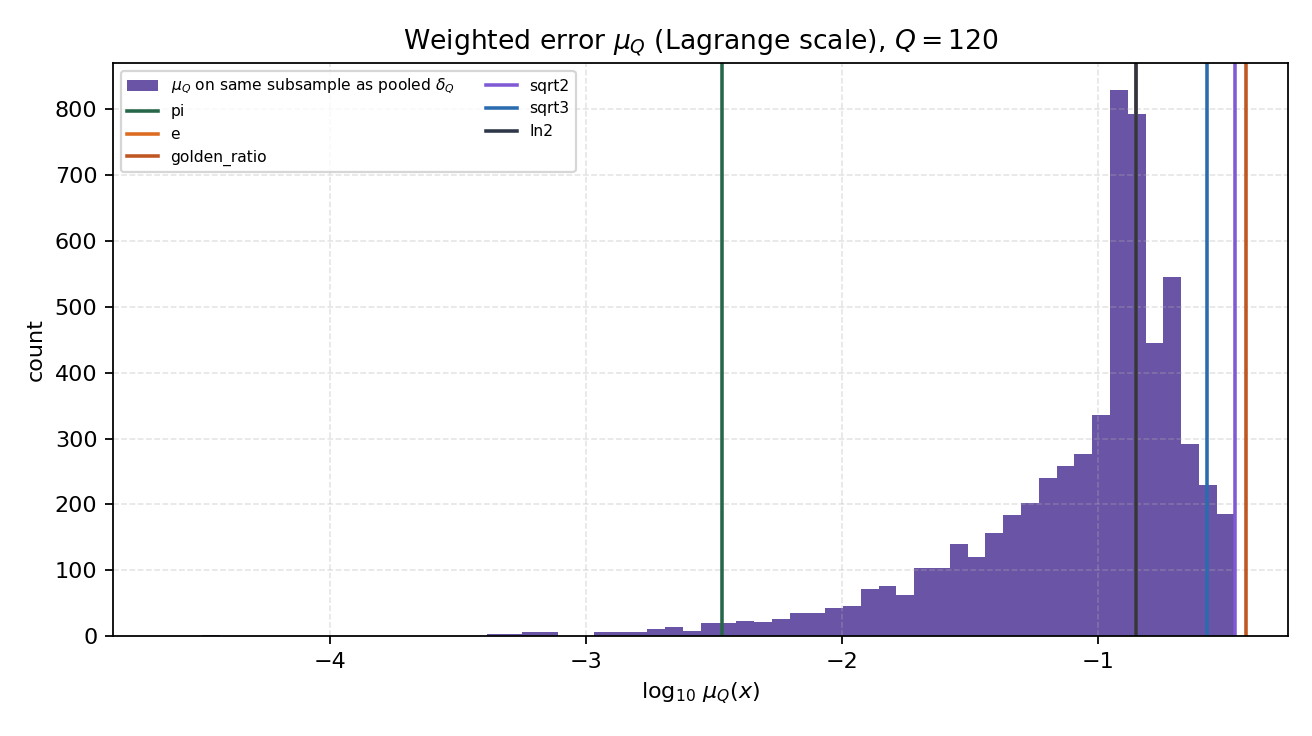
\includegraphics[keepaspectratio,alt={Figure. Histogram of \textbackslash log\_\{10\}\textbackslash mu\_Q(x) on the identical subsample as Figure  (Q=120, same seed and bin count). Vertical lines mark \textbackslash mu\_\{120\}(x\^{}\textbackslash star) for the same six constants. Interpreting this panel alongside Figures -- separates raw closeness \textbackslash delta\_Q from denominator-weighted quality \textbackslash mu\_Q; a constant can sit near the \textbackslash delta\_Q median while lying in an extreme \textbackslash mu\_Q tail if its best admissible approximant is comparatively weak on the q\^{}2 scale.}]{../figures/proximity_histogram_mu.png}}
\caption{\textbf{Figure.} Histogram of \(\log_{10}\mu_Q(x)\) on the
\textbf{identical} subsample as Figure \ref{fig:proximity_pooled}
(\(Q=120\), same seed and bin count). Vertical lines mark
\(\mu_{120}(x^\star)\) for the same six constants. Interpreting this
panel alongside Figures
\ref{fig:proximity_hist}--\ref{fig:proximity_pooled} separates raw
closeness \(\delta_Q\) from denominator-weighted quality \(\mu_Q\); a
constant can sit near the \(\delta_Q\) median while lying in an extreme
\(\mu_Q\) tail if its best admissible approximant is comparatively weak
on the \(q^2\) scale.}\label{fig:proximity_mu}
\end{figure}

\subsection{Related checks}\label{related-checks}

Lattice versus brute-force agreement is recorded in
\texttt{output/data/lattice\_crosscheck.json} from
\texttt{scripts/02\_lattice\_crosscheck.py}.

\newpage

\section{Conclusion}\label{conclusion}

Finite-\(Q\) rational proximity is a deliberately coarse lens: it
rewards numbers that admit unusually accurate low-height approximants,
not ``randomness'' in a probabilistic sense. Reporting \textbf{both}
\(\delta_Q\) and \(\mu_Q\) (\texttt{03e\_q\_squared\_quality.md})
separates raw closeness from denominator-weighted quality and catches
cases---such as the golden ratio in the default run---where the two
scales tell different stories at the same \(Q\).

At \(Q=120\) under the default pooled reference, \(\pi) occupies an
extreme left tail for \(\delta_Q\) while several algebraic irrationals
and transcendentals fall closer to the bulk; \texttt{q\_sensitivity}
shows that such rankings are \textbf{not monotone} in \(Q\) because
enlarging the rational search set can unlock new approximants in a
non-uniform way. Optional \texttt{compare\_mod1:\ true} re-expresses
constants on \([0,1)\) when the scientific question targets
uniform-on-the-circle comparison.

The pipeline remains modular (\texttt{src/continued\_fractions},
\texttt{rational\_distance}, \texttt{diophantine\_bounds},
\texttt{cf\_distance}, \texttt{sampling}, \texttt{statistics\_compare}),
tested without mocks (\texttt{docs/testing\_philosophy.md}), and
parameterized from \texttt{manuscript/config.yaml}. Figures subsample
for clarity; tables and JSON ranks reflect the \textbf{full} pooled
Monte Carlo array.

\newpage

\section{Reproducibility}\label{reproducibility}

\subsection{Software}\label{software}

\begin{itemize}
\tightlist
\item
  Python \(\geq 3.10\), NumPy, Matplotlib, PyYAML (declared in
  \texttt{projects/special\_number\_proximity/pyproject.toml}; root
  \texttt{uv\ sync} supplies the environment).
\item
  Tests:
  \texttt{uv\ run\ pytest\ projects/special\_number\_proximity/tests/\ -\/-cov=projects/special\_number\_proximity/src\ -\/-cov-fail-under=90}.
\end{itemize}

\subsection{Regenerating artifacts}\label{regenerating-artifacts}

\begin{Shaded}
\begin{Highlighting}[]
\ExtensionTok{uv}\NormalTok{ run python projects/special\_number\_proximity/scripts/proximity\_monte\_carlo.py}
\CommentTok{\# Optional: alternate project root (e.g. temporary checkout)}
\ExtensionTok{uv}\NormalTok{ run python projects/special\_number\_proximity/scripts/proximity\_monte\_carlo.py }\AttributeTok{{-}{-}project{-}dir}\NormalTok{ /path/to/projects/special\_number\_proximity}
\end{Highlighting}
\end{Shaded}

The script prints absolute paths to \textbf{five} outputs: JSON summary,
CSV constant table, and three PNG figures
(\texttt{proximity\_histogram.png},
\texttt{proximity\_histogram\_pooled.png},
\texttt{proximity\_histogram\_mu.png}).

Edits to \texttt{manuscript/config.yaml} under \texttt{experiment:}
change seeds, sample sizes, \texttt{q\_max},
\texttt{quadratic\_candidates}, \texttt{compare\_mod1},
\texttt{q\_sensitivity}, \texttt{histogram\_uniform\_cap}, and Beta
parameters without editing Python.

\subsection{Data paths}\label{data-paths}

{\def\LTcaptype{none} % do not increment counter
\begin{longtable}[]{@{}
  >{\raggedright\arraybackslash}p{(\linewidth - 2\tabcolsep) * \real{0.6250}}
  >{\raggedright\arraybackslash}p{(\linewidth - 2\tabcolsep) * \real{0.3750}}@{}}
\toprule\noalign{}
\begin{minipage}[b]{\linewidth}\raggedright
Artifact
\end{minipage} & \begin{minipage}[b]{\linewidth}\raggedright
Path
\end{minipage} \\
\midrule\noalign{}
\endhead
\bottomrule\noalign{}
\endlastfoot
Summary JSON &
\texttt{projects/special\_number\_proximity/output/data/proximity\_summary.json} \\
Table CSV &
\texttt{projects/special\_number\_proximity/output/data/proximity\_constants.csv} \\
Uniform \(\delta_Q\) histogram &
\texttt{projects/special\_number\_proximity/../figures/proximity\_histogram.png} \\
Pooled \(\delta_Q\) histogram &
\texttt{projects/special\_number\_proximity/../figures/proximity\_histogram\_pooled.png} \\
Pooled \(\mu_Q\) histogram &
\texttt{projects/special\_number\_proximity/../figures/proximity\_histogram\_mu.png} \\
Lattice cross-check &
\texttt{projects/special\_number\_proximity/output/data/lattice\_crosscheck.json} \\
\end{longtable}
}

Run
\texttt{uv\ run\ python\ projects/special\_number\_proximity/scripts/02\_lattice\_crosscheck.py}
to refresh the lattice JSON.

\subsection{Combined manuscript build}\label{combined-manuscript-build}

\begin{Shaded}
\begin{Highlighting}[]
\ExtensionTok{uv}\NormalTok{ run python scripts/03\_render\_pdf.py }\AttributeTok{{-}{-}project}\NormalTok{ special\_number\_proximity}
\ExtensionTok{python3} \AttributeTok{{-}m}\NormalTok{ infrastructure.validation.cli markdown projects/special\_number\_proximity/manuscript/}
\end{Highlighting}
\end{Shaded}

Authoring conventions for Markdown and cross-refs:
\href{../docs/manuscript_conventions.md}{\texttt{docs/manuscript\_conventions.md}}.

\newpage

\section{Limitations}\label{limitations}

\begin{itemize}
\item
  \textbf{Fixed \(Q\):} The statistics \(\delta_Q\) and \(\mu_Q\)
  (\eqref{eq:delta}, \eqref{eq:lagrange}) are evaluated at a single
  ceiling in the headline table (or a short list via
  \texttt{experiment.q\_sensitivity} in \texttt{config.yaml}). They do
  not classify a number's Diophantine type as \(Q \to \infty\).
\item
  \textbf{Reference law:} Empirical percentiles depend on the mixture of
  Uniform\((0,1)\), quadratic-mod-\(1\), and optional Beta draws.
  Changing \texttt{quadratic\_candidates} or sample sizes shifts the
  pooled CDF; \texttt{compare\_mod1:\ true} re-expresses constants on
  \([0,1)\) for fairer comparison when the uniform component dominates
  the scientific question.
\item
  \textbf{Histograms vs tables:} Figures use a capped
  \textbf{visualisation subsample} that omits Beta draws even when the
  pooled Monte Carlo includes them (\texttt{histogram\_uniform\_cap},
  see \texttt{03c\_monte\_carlo\_design.md}). JSON/CVS percentiles
  always use the full pooled array.
\item
  \textbf{Labels:} \texttt{NumberClass} tags in \texttt{constants.py}
  are documentary; the code does not certify transcendence or
  algebraicity.
\item
  \textbf{Convergent-only helper:}
  \texttt{min\_distance\_among\_convergents} can exceed \(\delta_Q\)
  when a semiconvergent beats every convergent with \(q \leq Q\).
\item
  \textbf{Floating point:} Results are IEEE-754 doubles. Pathological
  \(x\) with enormous partial quotients are not representative of the
  registry constants but illustrate that continued-fraction diagnostics
  can truncate early.
\end{itemize}

\newpage

\section{Notation and symbols}\label{notation-and-symbols}

{\def\LTcaptype{none} % do not increment counter
\begin{longtable}[]{@{}
  >{\raggedright\arraybackslash}p{(\linewidth - 2\tabcolsep) * \real{0.4706}}
  >{\raggedright\arraybackslash}p{(\linewidth - 2\tabcolsep) * \real{0.5294}}@{}}
\toprule\noalign{}
\begin{minipage}[b]{\linewidth}\raggedright
Symbol
\end{minipage} & \begin{minipage}[b]{\linewidth}\raggedright
Meaning
\end{minipage} \\
\midrule\noalign{}
\endhead
\bottomrule\noalign{}
\endlastfoot
\(Q\) & Fixed maximum denominator in \eqref{eq:delta}; integer
\(\geq 1\). \\
\(\delta_Q(x)\) & \(\min_{1\le q\le Q}\min_{p\in\mathbb{Z}} |x-p/q|\);
primary proximity statistic. \\
\(\mu_Q(x)\) & \(\min_{1\le q\le Q}\min_{p\in\mathbb{Z}} q^2|x-p/q|\);
Lagrange-type weighted error (\eqref{eq:lagrange}). \\
\(\|y\|\) & Distance from real \(y\) to the nearest integer. \\
\(\{x\}\) & Fractional part \(x-\lfloor x\rfloor\) (used when
\texttt{compare\_mod1} is enabled). \\
Pooled sample & Concatenation of configured uniform,
quadratic-mod-\(1\), and optional Beta draws on \([0,1)\) with one
shared RNG seed. \\
Empirical rank & Proportion of pooled draws with \(\delta_Q(X_i)\) (or
\(\mu_Q(X_i)\)) \textbf{strictly less} than the constant's value. \\
\texttt{q\_sensitivity} & YAML-driven list of extra \(Q\) values;
recomputes tables on the \textbf{same} pooled abscissa. \\
\end{longtable}
}

Module names refer to \texttt{projects/special\_number\_proximity/src/}
unless a path is explicit.

\newpage

\section{Reader's guide to registered
constants}\label{readers-guide-to-registered-constants}

Each entry below mirrors \texttt{src/constants.py}. Classification
strings are \textbf{informative only}; no formal proof is recomputed in
software.

\textbf{\texttt{pi} --- transcendental (documentary).} Circle constant.
Famous rational approximants at moderate height (e.g.~\(355/113\)) can
make \(\delta_Q\) extremely small at finite \(Q\) when those
denominators enter the search range.

\textbf{\texttt{e} --- transcendental (documentary).} Base of the
natural logarithm. Continued-fraction coefficients are unbounded;
finite-\(Q\) behaviour is read from the JSON after each run.

\textbf{\texttt{sqrt2}, \texttt{sqrt3} --- irrational algebraic degree
\(2\).} Quadratic irrationals are badly approximable in the classical
sense; nonetheless \(\delta_Q\) and \(\mu_Q\) at fixed \(Q\) depend on
which rational with \(q\le Q\) wins the minimum.

\textbf{\texttt{golden\_ratio} --- \(\varphi=(1+\sqrt5)/2\), quadratic
irrational.} All partial quotients equal \(1\) in exact
continued-fraction theory; expect bounded-quotient heuristics to
interact with \(\mu_Q\) ranks differently from \(\delta_Q\) ranks at the
same \(Q\).

\textbf{\texttt{ln2} --- transcendental (documentary).} Natural
logarithm of \(2\); included to show a transcendental on \((0,1)\)
alongside uniform-style references.

\textbf{\texttt{one\_sixth} --- rational control.} Exact value \(1/6\);
\(\delta_Q=\mu_Q=0\) for \(Q\ge 6\) under exact arithmetic. Serves as a
zero baseline for the scan and CSV export.



\bibliography{references}
\end{document}
